\documentclass[12pt]{article}
%\usepackage[backend=biber]{biblatex}
\usepackage{amsmath}
\usepackage{listings}
\usepackage{graphicx}
\usepackage{caption}
\usepackage{subcaption}
\usepackage{commath}
\usepackage{hyperref}
\usepackage{url}
\usepackage{xcolor}
\usepackage{textcomp}
\usepackage{dirtytalk}
\usepackage{listings}
\usepackage{wasysym}
\usepackage{float}
\usepackage{listings}
\usepackage[linesnumbered,lined,boxed,commentsnumbered]{algorithm2e}

% Packages from derivations_fullproblem.tex
\usepackage[squaren]{SIunits}
\usepackage{a4wide}
\usepackage{array}
\usepackage{cancel}
\usepackage{amsmath}
\usepackage{amsfonts}
\usepackage{amssymb}
\usepackage{graphicx}
\usepackage{enumerate}

% Parameters for displaying code.
\lstset{language=C++}
\lstset{basicstyle=\ttfamily\small}
\lstset{frame=single}
\lstset{keywordstyle=\color{red}\bfseries}
\lstset{commentstyle=\itshape\color{blue}}
\lstset{showspaces=false}
\lstset{showstringspaces=false}
\lstset{showtabs=false}
\lstset{breaklines}

% Define new commands
\newcommand{\expect}[1]{\langle #1 \rangle}

% Add bibliography
\begin{document}


\title{MAT4110 - Oblig 1}
\author{Geir Tore Ulvik - ulvik}
\maketitle

\section{Introduction}
The aim of this work is to implement two different methods for solving
the least squares problem for a linear set of equations. The first method
uses QR factorization to find the set of coefficients of the fitted polynomial $p$,
while the second method uses Cholesky factorization.
Differences between the methods are discussed.

The implementation is available at GitHub: 
\href{https://github.com/geirtul/mat4110/tree/master/oblig1}{GitHub Link}
\section{Discussion of the Methods}
The condition numbers listed in \ref{tab:condition} are rather high for the second
dataset, especially for $m = 8$ where it doesn't really make sense.
Unfortunately there wasn't time to further investigate the reason for these high numbers.
Fellow students taking this subject report lower, more reasonable numbers.
\begin{table}[h]
\center
\begin{tabular}{c c c}
	Method & m & Condition number \\
	\hline
	QR & $3$ & $7.78$ \\
	Cholesky & $8$ & $60.53$\\
	QR & $3$ & $1544.43$ \\
	Cholesky & $8$ & $2385272.75$\\
\end{tabular}
	\caption{Condition numbers for the vandermonde matrices associated with the problems
		related to each dataset, using the Euclidian norm. 
		$m$ is the order of the fitted polynomial.}
\label{tab:condition}
\end{table}

However, ignoring the size of the number, the trend is still clear. For the Cholesky
method the condition number is the condition for the QR method squared.
This makes sense as the condition number is related to the problem itself, and in
the Cholesky method we solve using the matrix $B = A^TA$, while QR used just $A$.
This naturally leads to the problem being more sensitive to perturbations in the input.

Other than that, comparing the plots of the fitted polynomials 
(\ref{fig:qr-3} vs. \ref{fig:cholesky-3} and \ref{fig:qr-8} vs. \ref{fig:cholesky-8}), 
the methods provide (visually) indistinguishable results.
Increasing the amount of noise in the dataset by varying 'eps' changes the fit
for both models, but they are still indistinguishable.

For this problem it then seems that choice of method is irrelevant. This might not
be the case for problems containing larger datasets and different conditions.
The QR-method is generally regarded as the more stable method when solving
the least squares problem, but the Cholesky approach can increase performance
if you can safely express your problem using a symmetric matrix. 

For the QR-method, three different algorithms for the factorization are available,
each with their own advantages/disadvantages, so depending on the problem one sets out
to solve, digging a little deeper into the underlying algorithms can be very beneficial.

\section{Figures}
\begin{figure}[h]
	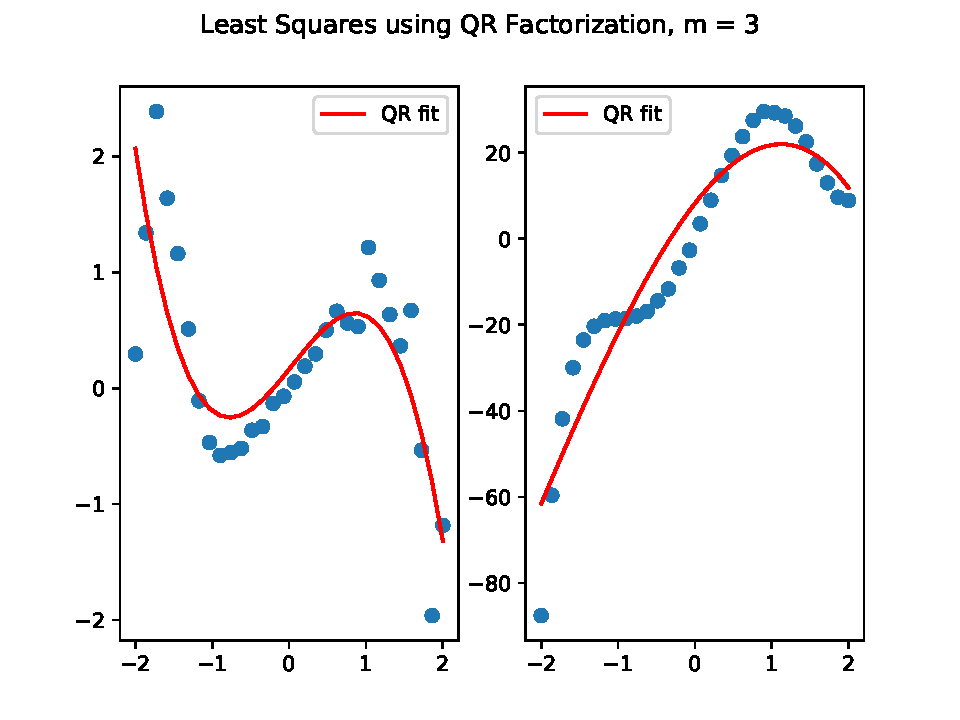
\includegraphics[width = \textwidth]{figures/QR_3.pdf}
	\caption{Plotted results of performing linear regression to solve the least squares
		problem using QR Factorization. The fitted polynomial is of degree 3.}
	\label{fig:qr-3}
\end{figure}
\begin{figure}[h]

	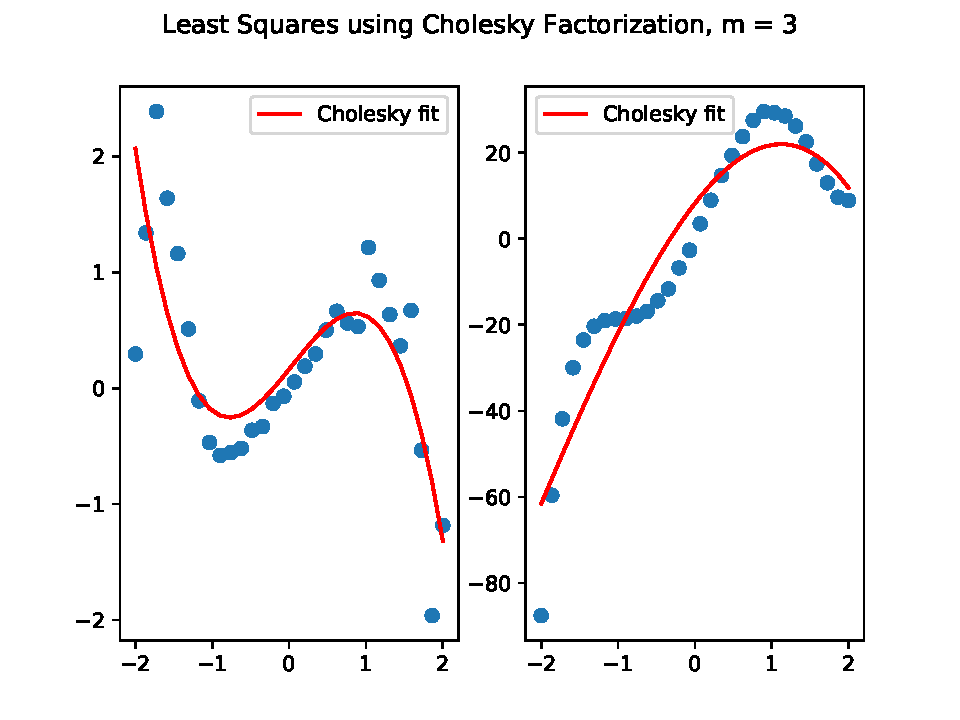
\includegraphics[width = \textwidth]{figures/Cholesky_3.pdf}
	\caption{Plotted results of performing linear regression to solve the least squares
		problem using Cholesky Factorization. The fitted polynomial is of degree 3.}
	\label{fig:cholesky-3}
\end{figure}
\begin{figure}[h]

	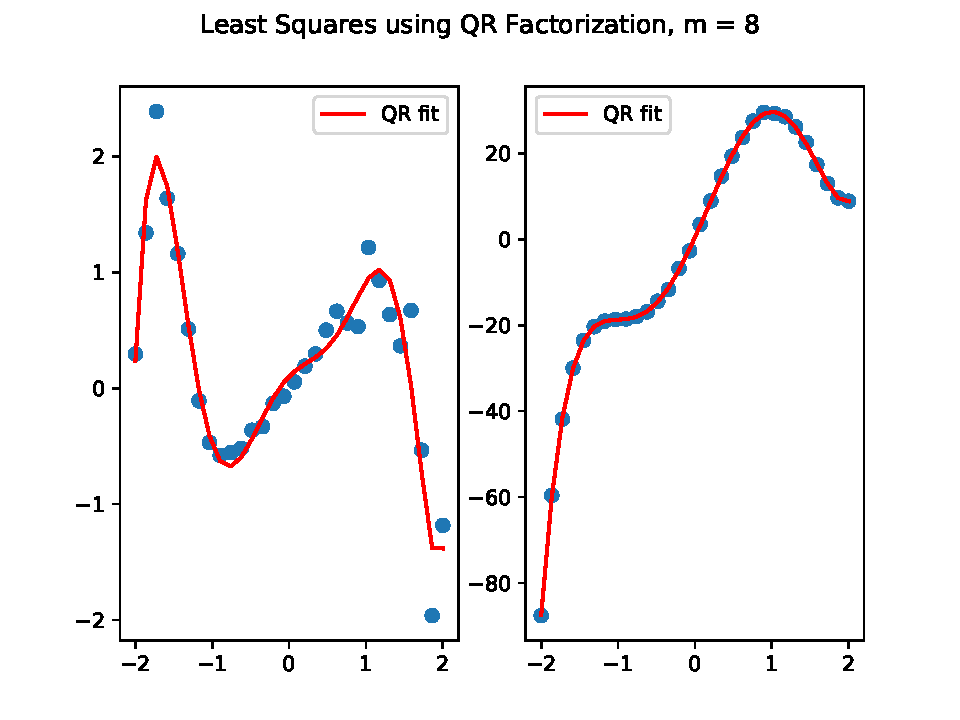
\includegraphics[width = \textwidth]{figures/QR_8.pdf}
	\caption{Plotted results of performing linear regression to solve the least squares
		problem using QR Factorization. The fitted polynomial is of degree 8.}
	\label{fig:qr-8}
\end{figure}
\begin{figure}[h]

	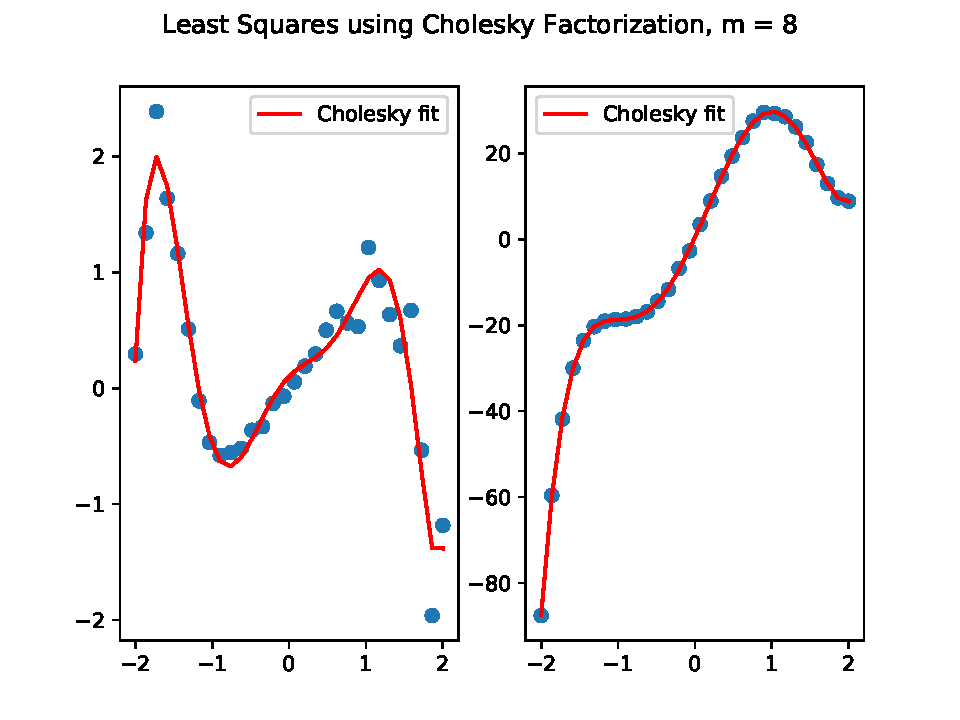
\includegraphics[width = \textwidth]{figures/Cholesky_8.pdf}
	\caption{Plotted results of performing linear regression to solve the least squares
		problem using Cholesky Factorization. The fitted polynomial is of degree 8.}
	\label{fig:cholesky-8}
\end{figure}


\end{document}
